\section*{Suggested Teaching Resources} 
\section*{Lesson \ref{limits}}
\begin{itemize}[leftmargin=*]
    \item Definition of the Derivative Geogebra Applet (\url{https://www.geogebra.org/m/F4Pu8PMt#material/NKFCBKCY}): This applet helps students:
    \begin{itemize}
        \item relate the average rate of change to the instantaneous rate of change and hence to the definition of the derivative;
        \item understand the difference between a secant line and a tangent line
    \end{itemize}
     
\end{itemize}

\section*{Lesson \ref{diffRules}}
\begin{itemize}[leftmargin=*]
    \item Example \ref{exHorzTang} 
    \begin{itemize}
        \item Intro to Desmos Tutorial videos:
        \begin{itemize}
            \item \url{https://youtu.be/7oVOs9TX57s}
            \item \url{https://youtu.be/En_PkyA-4_4} 
        \end{itemize}
        \item Use Desmos to graph the function $f$ and the horizontal tangent lines:
        \begin{figure}[h!]
        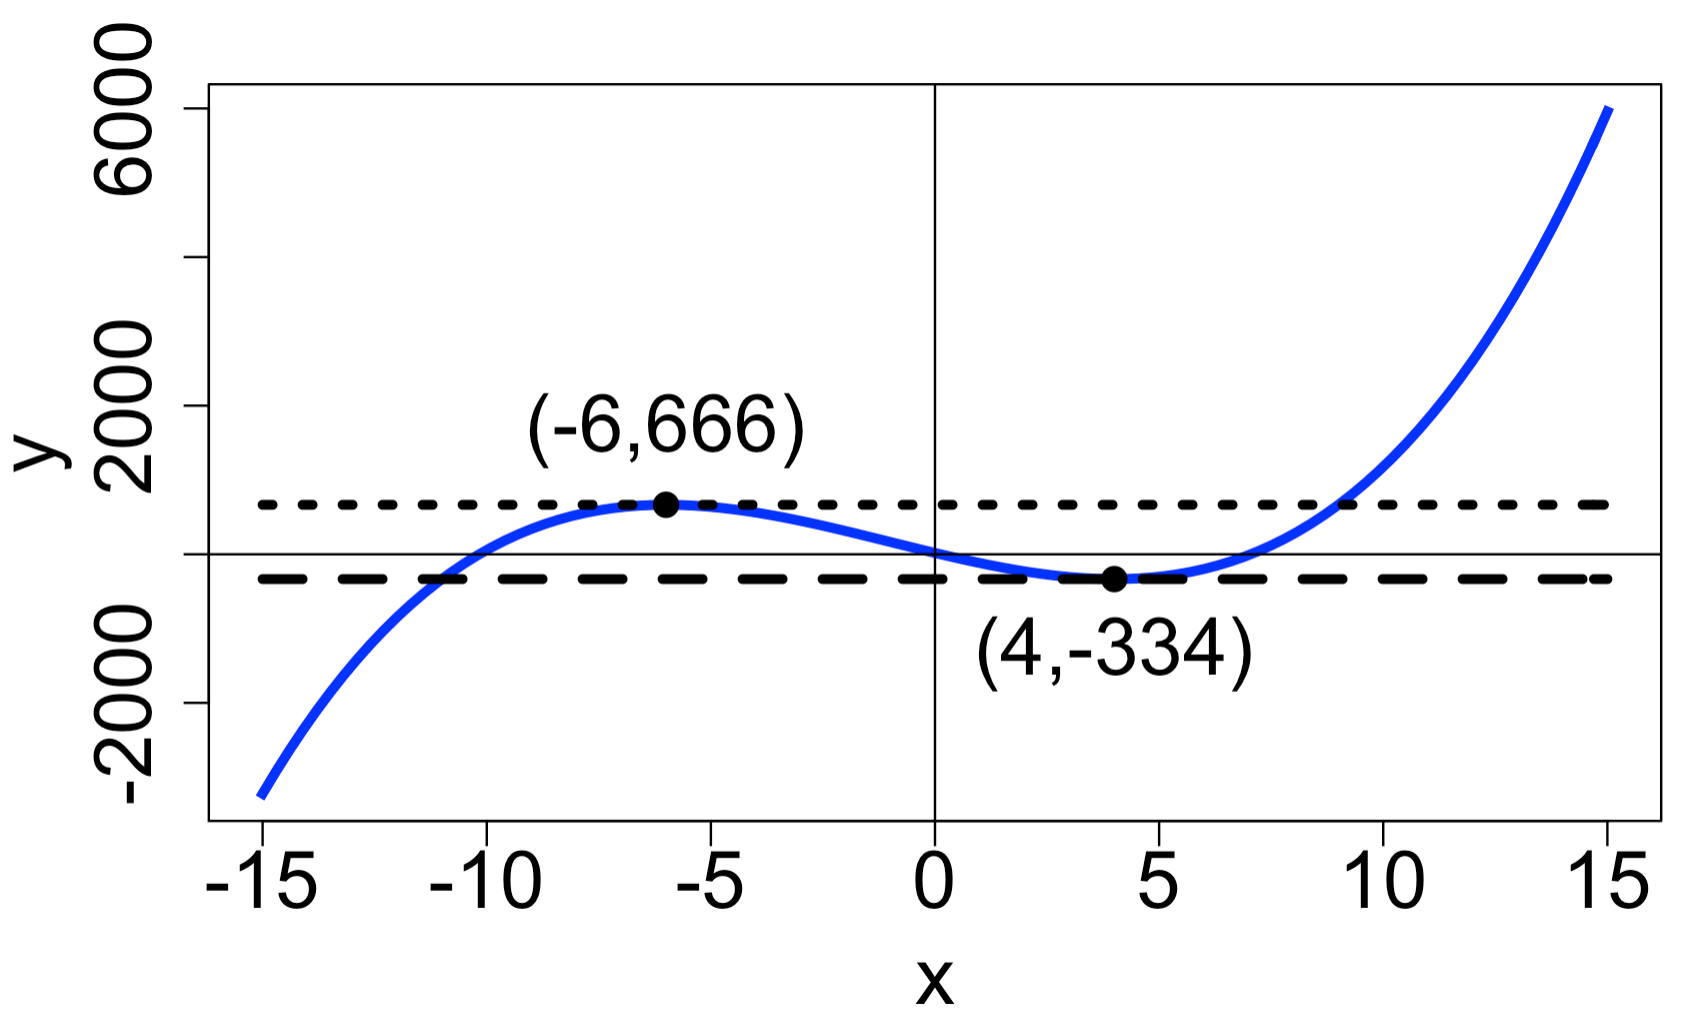
\includegraphics[width=0.5\textwidth,inner]{images/differentiationRules/Lesson4_HorizontalTangentEx.png}
        \end{figure}
    \end{itemize}
    
     
\end{itemize}

\section*{Lesson \ref{GenPower}}
\begin{itemize}[leftmargin=*]
    \item Use an animation of the chain rule to help intuitively understand the notation of the chain rule. 
    \begin{itemize}
        \item \url{http://webspace.ship.edu/msrenault/GeoGebraCalculus/derivative_intuitive_chain_rule.html}
    \end{itemize}
     
\end{itemize}